\documentclass{article} 
\usepackage[utf8]{inputenc}
\usepackage{amsmath}  
\usepackage{graphicx}
\usepackage{caption}  
\usepackage{enumitem}
\usepackage{lipsum} 
\usepackage[T1]{fontenc}

\title{Pixlel}
\author{Kinga Kowal}
\date{November 2023}

\begin{document}

\maketitle

\section{Wyrażenie matematyczne}
\[ (a+b)^3=a^2+2ab+b^2 \]

\section{Lista nienumerowana}
\begin{itemize}
  \item jeden
  \item trzy
  \item siedem
\end{itemize}

\section{Numerowana}
\label{sec:lista}
\begin{enumerate}
  \item dwa
  \item pięć
  \item sześć
\end{enumerate}



\begin{figure}
    \centering
    \centerline{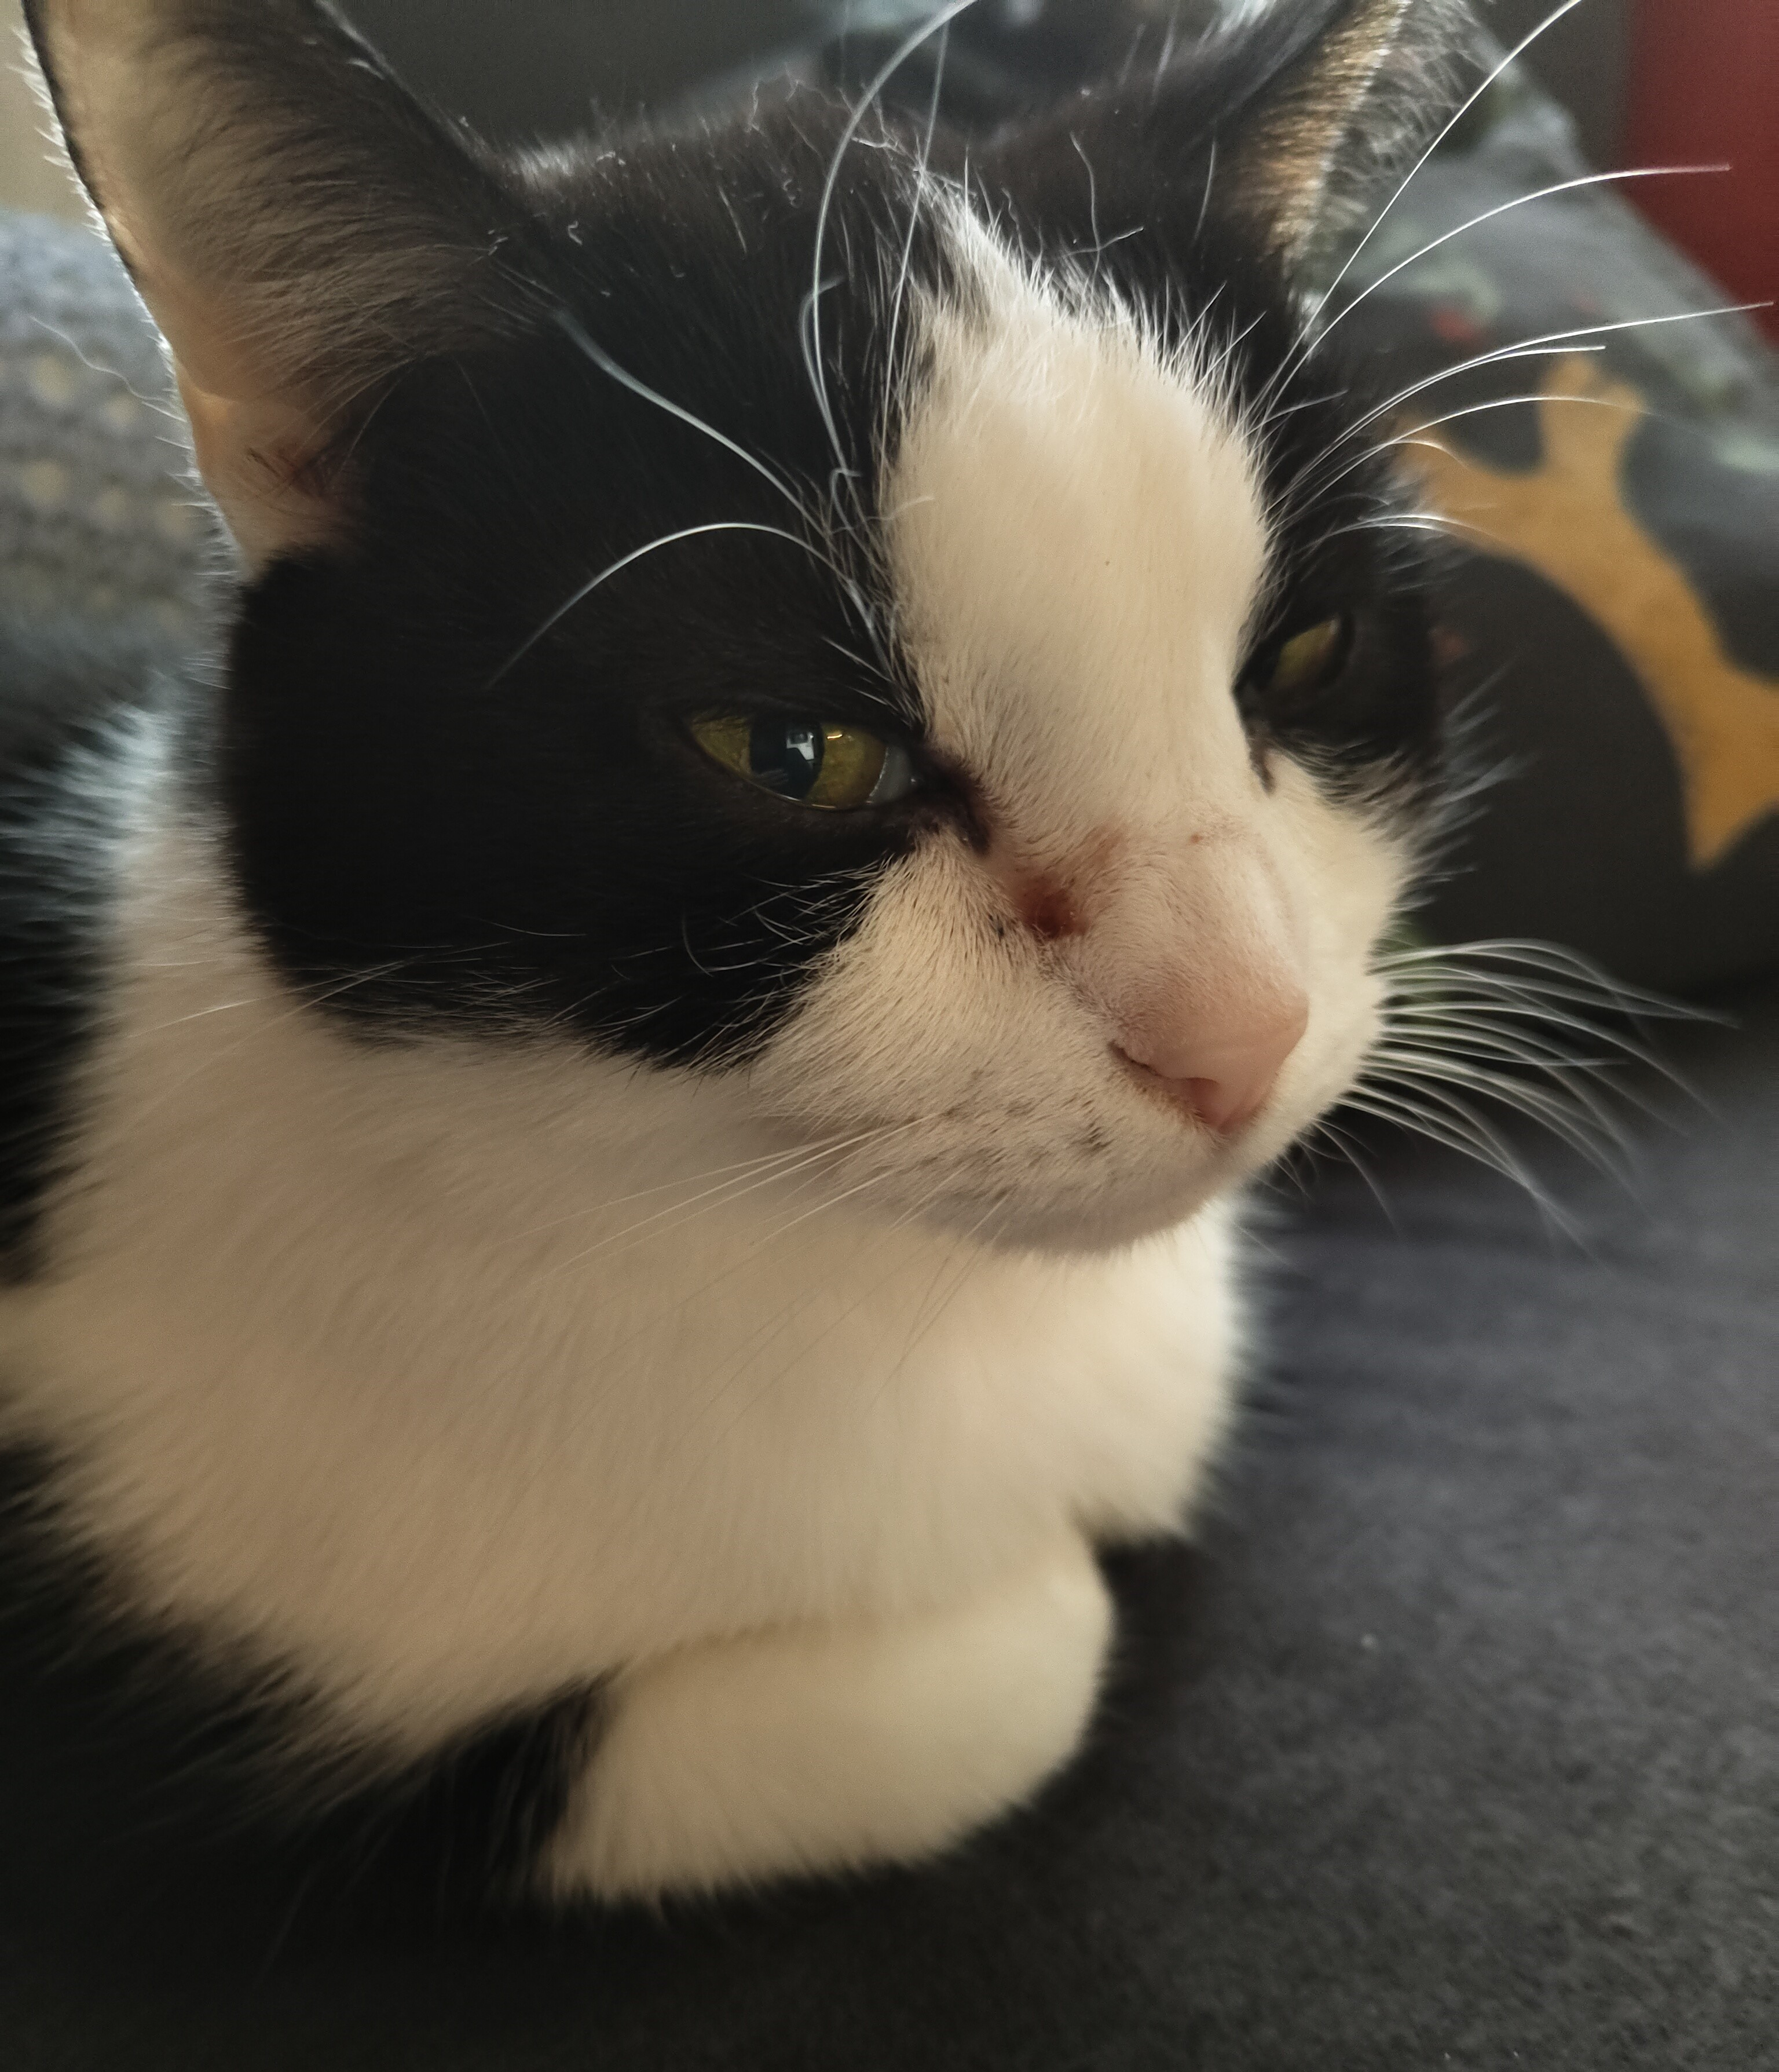
\includegraphics[scale=0.15]{pictures/kow.jpg}}
    \caption[width=0.4\textwidth]{Zdjecie}
    \label{Zdjecie kota}
\end{figure}


\begin{table}[]
\centering
\caption{Tabela}
\begin{tabular}{|l|l|l|l|l|}
\hline
  & a & b & c  & d  \\ \hline
1 & 1 & 1 & 1  & 1  \\ \hline
2 & 2 & 4 & 8  & 16 \\ \hline
3 & 3 & 9 & 27 & 81 \\ \hline
\end{tabular}
\label{tab:kkow}
\end{table} 

\textbf{Litoria majikthise}- \emph{gatunek} indonezyjskiego \emph{podrodziny Litoriinae w rodzinie Pelodryadidae} \ref{tab:kkow}. 

\textbf{\emph{Status}} i tendencje trudno jest określić, aczkolwiek wydaje się, że lokalnie występować mogą tendencje zniżkowe \ref{sec:lista}.
\end{document}